\section{Working with \rt transit data}
\label{sec:gtfs}


GTFS (general transit feed specification)
is an API (application programming interface) specification for transit data
detailing how it should be organised,
making access easier for application developers.
GTFS, developed and maintained by Google \citep{GoogleDevelopers_2006},
% who use it in Google Maps Transit Directions,
is used by over 1100~transit providers around the world
(sourced from \url{http://transitfeeds.com} on August 2019),
including here in Auckland, New Zealand.
An advantage of this standardised format is that,
provided an application depends solely on GTFS data,
after developing it locally in Auckland it will be deployable to any other GTFS-based
public transport system with minimal modification.


There are two components to GTFS.
The first, \emph{GTFS static}, includes information about:
\begin{itemize}
\item \emph{stops}, a physical location where passengers can embark and disembark the vehicle;
\item \emph{routes}, a sequence of two or more stops displayed as a single service;
\item \emph{trips}, an instance of a route occurring at a specific time of day;
\item \emph{schedules}, specifying the arrival (and departure) times for each bus at each of its stops;
\item and \emph{shapes}, the sequence of points defining a vehicle's path along a route.
\end{itemize}
The second component, \emph{GTFS-realtime},
is only available in a subset of providers due to the requirement of
on-board GPS tracking devices and a central server.
It provides a standardised format for sharing vehicle positions and trip delays,
which developers access via an API for use in \rt applications.

As mentioned in Section~\ref{sec:intro},
there are some fundamental issues with the arrival time prediction method currently
deployed in Auckland,
which is based entirely on \emph{GTFS-realtime} trip updates---%
vehicle positions are used only to display \emph{where} the bus is.
Vehicles report a trip update,
which includes the delay between scheduled and actual arrival time,
when they arrive at or depart from a stop.
The delay is then propagated to all future stops to update their ETAs,
as demonstrated in Figure~\ref{fig:gtfs-delays}.
As already mentioned, this assumes that the schedule is well-calibrated
and that the time between stops
is representative of the real-world travel time between them.
Figure~\ref{fig:gtfs-delays} demonstrates the fallibility of this prediction method,
where we see the incremental lateness causing the passenger's ETA to
jump each time the bus arrives at a stop.
By using \rt travel time information,
we can better predict the travel time between stops,
from which more accurate and, ideally, more reliable arrival esimates
can be made.


\begin{figure}[tb]
    \centering
    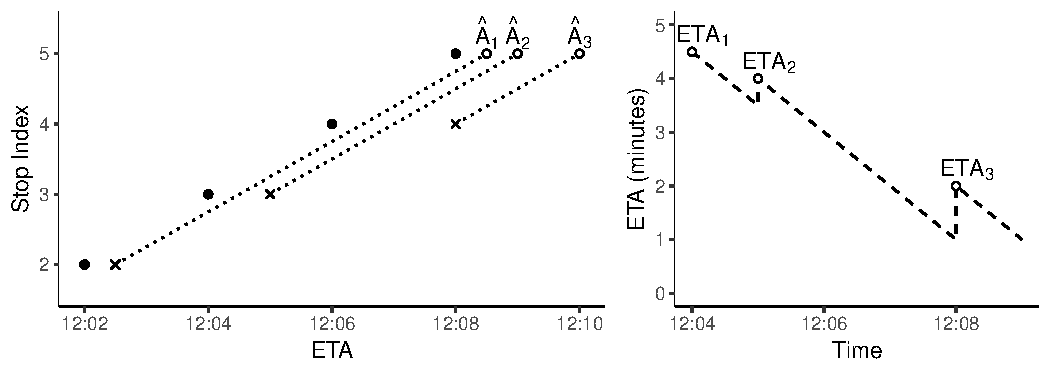
\includegraphics[width=0.8\textwidth]{figures/02_gtfs_delays.pdf}
    \caption{
        On the left, scheduled arrival times are shown as solid points,
        for several stops along a route. The actual arrival times
        are shown with crosses,
        and the GTFS-based ETAs for stop 5, $\{\hat A_1, \hat A_2, \hat A_3\}$, are shown.
        On the right,
        for a passenger arriving at stop 5 at 12:04,
        ETA predictions
        $\mathrm{ETA}_j = \mathrm{Time} - \hat A_j$ are shown
        to demonstrate the fluctuation in
        arrival time as the bus arrives at each stop.
    }
    \label{fig:gtfs-delays}
\end{figure}



\subsection{Transit network construction}
\label{sec:network_build}

The primary predictor of arrival time is
the travel time along roads between where the bus is \emph{now},
and the stop where a passenger waits.
In most applications, however, this vital information is unavailable, at least directly.
In order to compute travel times efficiently
and make use of all available data pooled across multiple routes,
we constructed a \emph{road network},
allowing us to model roads directly,
such that every bus travelling along a road contributes to its state,
which can, in turn, be used to predict travel times for all upcoming buses
travelling along the same road,
irrespective of the route they are servicing.


Constructing the transit network involved splitting routes
into spatially identifiable segments,
each representative of a physical road,
using bus stops as nodes in the network
and the connecting roads as edges
(Figure~\ref{fig:network_creation}).
In this way, routes that service the same subsequence of stops
all contribute to traffic flow information for the connecting roads.
Although there are several drawbacks to this method,
such as road segment overlaps where routes merge between stops,
our approach is sufficient for assessing the \rt
feasibility of our proposed prediction framework.



\begin{figure}[tb]
    \centering
    \begin{subfigure}{0.7\textwidth}
        \centering
        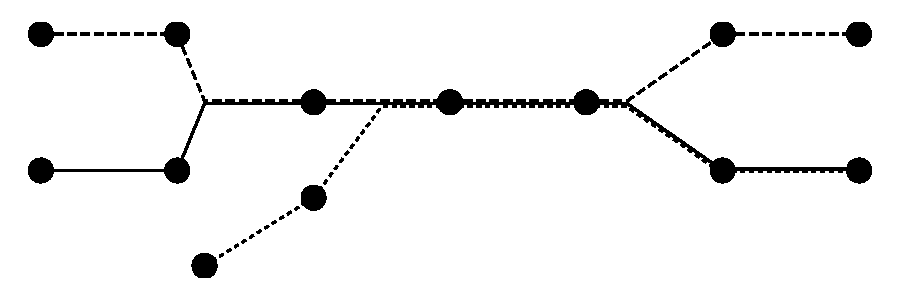
\includegraphics[width=0.9\textwidth]{figures/02_network_segments_1.pdf}
        \caption{Raw GTFS route shapes}
        \label{fig:network_creation_1}
    \end{subfigure} \\
    \begin{subfigure}{0.7\textwidth}
        \centering
        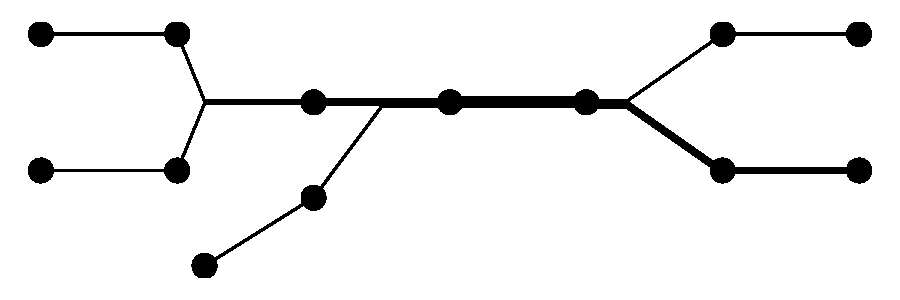
\includegraphics[width=0.9\textwidth]{figures/02_network_segments_2.pdf}
        \caption{GTFS-based road network}
        \label{fig:network_creation_2}
    \end{subfigure}
    \caption{
        Bus stops (shown as dots above) can be serviced by more than one route,
        as shown in (a), with different line types representing three separate routes.
        The constructed road network, using stops as nodes, is shown in (b),
        in which the connecting lines represent physical road segments,
        with line width proportional to the number of individual routes
        travelling along that road.
    }
    \label{fig:network_creation}
\end{figure}


\subsection{Real-time vehicle locations}
\label{sec:realtime_data}

\emph{GTFS-realtime} provides the positions of vehicles in a transit network.
The data consists of the time $t_k$ that the position was last updated,
the GPS position of the vehicle, $\bY_k$,
and information about the serviced trip.
In Auckland, vehicle positions are updated with a frequency
of anywhere between 10~seconds and several minutes,
so there is often considerable uncertainty about a vehicle's intermediate trajectory,
in particular when there are one or more bus stops along the way.
It is also possible for a bus to remain stationary,
such as when there is heavy congestion,
so the number of possible trajectories rapidly increases with
the time between observations.


An important consideration regarding Auckland Transport's \rt implementation is that
buses are programmed to report their location when arriving at or departing from
bus stops, as well as some major intersections.
To further complicate this,
these positions can be pre-emptive,
for example when approaching a queue of traffic at an intersection:
the way-point may trigger before the bus physically gets to it,
so consecutive observations may show what appears to be a bus travelling backwards.
To handle this, we compute the approximate distance travelled, $\tilde x_k$,
of the vehicle by finding the nearest point on the path to the observation;
if this has decreased, we reject the current state (based on the pre-emptive observation)
and reset the vehicle
to its previous state before continuing.
So at the cost of losing one (likely invalid) observation,
we can improve predictive performance
when this event occurs.
